\documentclass[12 pt, russian]{article}
\usepackage[T1]{fontenc}
\usepackage{ulem}
\usepackage[utf8]{luainputenc}
\usepackage{geometry}
\usepackage[pdftex]{graphicx}
\geometry{verbose,tmargin=3cm,bmargin=3cm,lmargin=3cm,rmargin=3cm}
\usepackage{amstext}
\usepackage{amsthm}
\usepackage{amssymb}
\usepackage{amsmath}
\usepackage[T1,T2A]{fontenc}
\usepackage[utf8]{inputenc}
\usepackage[english,main=russian]{babel}
\usepackage{setspace}
\usepackage{esint}
\usepackage{comment}
\usepackage{babel}
\usepackage{float}
\usepackage{amsfonts}
\usepackage{fullpage} 
\usepackage{parskip} 
\usepackage{tikz} 
\usepackage{indentfirst}

\def\hbr{\hfil\break}
\newcommand\F{\mbox{I\kern-2pt F}}
\newcommand\cA{{\cal A}}
\newcommand\cE{{\cal E}}
\newcommand\cC{{\cal C}}
\newcommand\cF{{\cal F}}
\newcommand\cG{{\cal G}}
\newcommand\cI{{\cal I}}
\newcommand\cK{{\cal K}}
\newcommand\cL{{\cal L}}
\newcommand\cB{{\cal B}}
\newcommand\cN{{\cal N}}
\newcommand\cM{{\cal M}}
\newcommand\cX{{\cal X}}
\newcommand\cD{{\cal D}}
\newcommand\cO{{\cal O}}
\newcommand\cR{{\cal R}}
\newcommand\cP{{\cal P}}
\newcommand\cQ{{\cal Q}}
\newcommand\cS{{\cal S}}
\newcommand\cT{{\cal T}}
\newcommand\cV{{\cal V}}
\newcommand\cY{{\cal Y}}
\newcommand\cZ{{\cal Z}}
\newcommand\R{\bbr}
\newcommand\uv{{\underline v}}
\newcommand\uw{{\underline w}}
\newcommand\up{{\underline p}}
\newcommand\uV{{\underline V}}
\newcommand\uW{{\underline W}}
\newcommand\bp{{\bar p}}
\newcommand\bv{{\bar v}}
\newcommand\bw{{\bar w}}
\newcommand\bV{{\bar V}}
\newcommand\bW{{\bar W}}
\def\bbr{{\mathbb R}}
\def\bbn{{\mathbb N}}
\def\bbc{{\mathbb C}}
\def\bbz{{\mathbb Z}}
\newcommand\e{{\varepsilon}}
\newtheorem{theo}{Theorem}[section]
\newtheorem{prop}[theo]{Proposition}
\newtheorem{lemm}[theo]{Lemma}
\newtheorem{coro}[theo]{Corollary}
\newtheorem{defin}[theo]{Definition}
\newtheorem{rem}[theo]{Remark}
\newcommand\fdem{$\Box$}
\newcommand\beq{\begin{equation}}
\newcommand\eeq{\end{equation}}
\newcommand\bea{\begin{eqnarray}}
\newcommand\eea{\end{eqnarray}}
\newcommand\bean{\begin{eqnarray*}}
	\newcommand\eean{\end{eqnarray*}}


\title{Курсовая работа ФИО}
\raggedbottom
\begin{document}
\thispagestyle{empty}
\newtheorem{Thm}{Теорема}[section]
\newtheorem{Lem}{Лемма}[section]
\newtheorem{Rem}{Замечание}[section]
\newtheorem{Co}{Следствие}[section]
\theoremstyle{definition}
\newtheorem{Exam}{Пример}[section]
\newtheorem{Dfn}{Определение}[section]
\sloppy
\begin{titlepage}
\begin{center}
Московский государственный университет имени~М.~В.~Ломоносова\\
Механико-математический факультет\\
Кафедра Теории Вероятностей\\
\centering
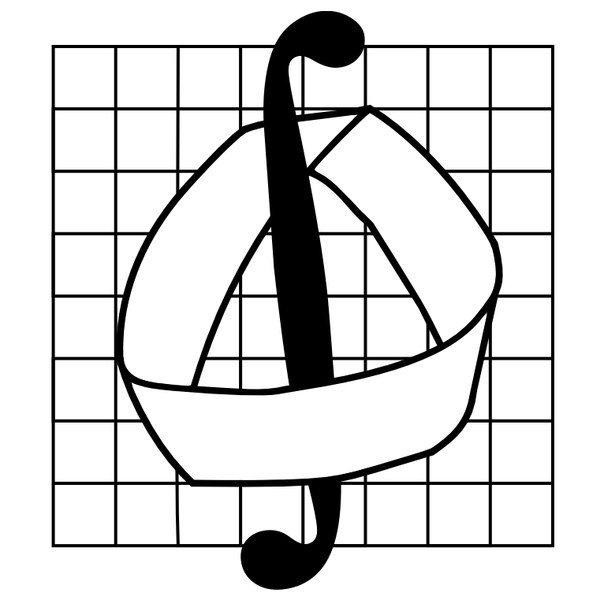
\includegraphics[width=0.3\textwidth]{mechmath.jpg}

\vspace*{100pt} Отчёт\\
студента 409 группы \\
Сидоренко Артура Павловича \\
\vspace{10pt} {\Large{\textbf{}}\\}
\textbf{Пять разностных схем для линейного однородного дифференциального уравнения первого порядка}
\vspace*{40pt}


\vspace*{\fill} Москва, 2020
\end{center}
\end{titlepage}

\section{Постановка задачи}
Дана задача Коши
\beq
y' + Ay = 0, y(0) = 1,
\eeq
где $y\colon \bbr \rightarrow \bbr$ , $A \in \bbr_+$. Известно, что тогда $y = e^{-Ax}$.  Для определённости положим и $x \in [0, 10]$.

Предлагается исследовать пять разностных схем для решения этого уравнения:
\bea
\frac{y_{k+1} - y_k}{h} + Ay_k = 0, y_0 = 1, \\
\frac{y_{k+1} - y_k}{h} + Ay_{k+1} = 0,   y_0 = 1,\\
\frac{y_{k+1} - y_k}{h} + A \frac{y_{k+1} + y_k}{2} = 0,  y_0 = 1,\\
\frac{y_{k+1} - y_{k-1}}{2h} + Ay_k = 0,   y_0 = 1, y_1 = y_0 - Ah,\\
\frac{1.5 y_{k+1} - 2 y_k + 0.5 y_{k-1}}{h} + Ay_k = 0,  y_0 = 1,  y_1 = y_0 - Ah.\\
\eea

У нас имеется дифференциальная задача с неизвестной в подпространстве достаточно гладких функций в $L_2$ и семейство разностных задач с параметром $h$ в пространствах $\bbr ^ {N(h)+1}$ с нормой $L(2, h)$, порождённым скалярным произведением вида $(f, g)_h = \sum{f_k g_k h}$. Пространства непрерывные и дискретные связаны между собой опреатором проектирования на дельта-функции: $(y)_h = ( y_k )_{k = 0 , \dots, N(h)}$,
$y_k = \int_\bbr{ \delta(x - x_k) y(x) dx}$, $x_k = x_0 + kh$.  Нетрудно видеть, что нормы в $L_2$ и $L(2, h)$ согласованы, так как норма $L(2, h)$ будет интегральной суммой Римана. 

Требуется провести исследование сходимости численного приближения задачи Коши к непрерывному решению. Именно, мы имеем численное решение $y^c_h \in \bbr^{1+N(h)}$ и точное решение $y(x)$. Надо проверить $||(y)_h - y^c_h||_h \leq Ch^p$, и с каким показателем $p$. 

\section{Теоретическое решение}

Я буду руководствоваться определениями в \cite{Kornev1}, стр. 254-259 и \cite{Kornev2}, стр.27-32.

\begin{theo}
Разностные схема (2) и (3) суть аппроксимации задачи (1) на решении с порядком 1.
\end{theo}
\begin{proof}
Остновимся на схеме (2). Проверим локальную аппрокимацию. По формуле Тейлора $y(x_{k+1}) = y(x_k) + y'(x_k) h + \frac{1}{2} y''(x_k) h^2 + \frac{1}{6} y'''(x_k + \xi) h^3$. Учитывая, что после проектирования $y_k = y(x_k)$, получим левую часть в (2) в виде 
\beq
y'(x_k) + y''(x_k) \frac{h}{2} + y'''(x_k + \xi) \frac{h^2}{6} + A y(x_k).
\eeq

Но на решении $y'(x_k) + Ay(x_k) = 0$, отсюда получаем, что левая часть в (2) будет равна $0.5 y''(x_k)h + O(h^2)$. Далее, так как при достаточно высокой гладкости $y''$ ограничена на $[0, 10]$, то мы получаем $||L_h (y)_h - 0||_h = O(h)$, где $L_h f = \frac{f_{k+1} - f_k}{h} + Af_k$. 
Начальные условия у нас точные, так что проверять их аппроксимацию не надо.
Для схемы (3) проверки абсолютно аналогичны.
\end{proof} 

\begin{theo}
Разностная схема (4) имеет второй порядок аппроксимации на решении.
\end{theo}
\begin{proof}
Аналогично с предыдущей теоремой, выпишем формулу Тейлора 
\beq
\label{t}
y(x_{k+1}) = y(x_k) + y'(x_k) h + \frac{1}{2} y''(x_k) h^2 + \frac{1}{6} y'''(x_k ) h^3 + \frac{1}{24} y^{IV}(x_k + \xi) h^4
\eeq
 и подставим в левую часть (4), приняв $y_k = y(x_k)$:
%\beq
\begin{multline}
y'(x_k) + y''(x_k) \frac{h}{2} + y'''(x_k) \frac{h^2}{6} + \frac{1}{24} y^{IV}(x_k + \xi) h^3 + A y(x_k) + \\  \frac{1}{2} A ( y'(x_k) h + \frac{1}{2} y''(x_k) h^2 +\frac{1}{6} y'''(x_k ) h^3 + \frac{1}{24} y^{IV}(x_k + \xi) h^4).
\end{multline}
%\eeq
Но на решении $y'(x_k) + Ay(x_k) = 0$ и $y''(x_k) + Ay'(x_k) = 0$. Тогда получаем 

\beq
y'''(x_k) \frac{h^2}{6} + \frac{1}{24} y^{IV}(x_k + \xi) h^3 + \frac{1}{2} A (\frac{1}{2} y''(x_k) h^2 +\frac{1}{6} y'''(x_k ) h^3 + \frac{1}{24} y^{IV}(x_k + \xi) h^4), 
\eeq
то есть $O(h^2)$. Аналогичные с предыдущим доказательством соображения приводят к  $||L_h (y)_h - 0||_h = O(h^2)$.
\end{proof}

\begin{theo}
Схемы (5) и (6) имеют второй и первый порядок аппроксимации соответственно.
\end{theo}
\begin{proof}
В (5) и (6) нужно проверять аппроксимации для $y_k$ и $y_1$ отдельно. Аппроксимация для $y_1$ имеет второй порядок. В (5) мы имеет аппроксимацию второго порядка для $y_k$. Посмотрим теперь на (6). Используя \ref{t} по аналогии с предыдущими выкладками, получим

\begin{multline}
y'(x_k) + \frac{1}{h}( y''(x_k)  h^2 + \frac{1}{6} y'''(x_k) h^3 + \frac{1}{24} (y^{IV}(x_k + \xi) +  y^{IV}(x_k + \eta)) h^4) +\\ A(y(x_k) - y'(x_k) h + \frac{1}{2} y''(x_k) h^2 - \frac{1}{6} y'''(x_k ) h^3 + \frac{1}{24} y^{IV}(x_k + \eta) h^4).
\end{multline}

После учёта $y' + Ay = 0$, будет

\begin{multline}
 \frac{1}{h}( y''(x_k)  h^2 + \frac{1}{6} y'''(x_k) h^3 + \frac{1}{24} (y^{IV}(x_k + \xi) +  y^{IV}(x_k + \eta)) h^4) +\\ A(- y'(x_k) h + \frac{1}{2} y''(x_k) h^2 - \frac{1}{6} y'''(x_k ) h^3 + \frac{1}{24} y^{IV}(x_k + \eta) h^4).
\end{multline}

Получаем в итоге $O(h)$.

\end{proof}

Теперь исследуем устойчивость решений. Схемы (2)-(6) суть линейные разностные уравнения, так что не надо использовать определение. Достаточно будет только лишь посмотреть на собственные значения: они все должны быть в единичном круге, а на единичной окружности не должно быть кратных. 
\begin{theo}
Схема (2) условно устойчива, т.е. устойчива при $h \leq 2/A$. Схемы (3) и (4) абсолютно устойчивы.
\end{theo}
\begin{proof}
Для (2) выпишем характеристический многочлен:
\beq
\frac{\lambda - 1}{h} + A = 0
\eeq.
Его корень
\beq
\lambda = 1 - Ah.
\eeq
Тогда $|\lambda| \leq 1$ т.т.т.к. $h \leq 2/A$.
В случае (3) получаем корень
\beq
\lambda = \frac{1}{1 + Ah},
\eeq
который всегда не превосходит единицы. В случае (4) имеем
\beq
\lambda = \frac{1 - 0.5Ah}{1 + 0.5Ah},
\eeq
что тоже не превосходит единицы по модулю.
\end{proof}

\begin{theo}
Схема (5) неустойчива.
\end{theo}
\begin{proof}
Имеем характеристический многочлен
\beq
\frac{\lambda^2 - 1}{h} - A\lambda = 0.
\eeq
Исследуя его корни, можно найти, что оба корня вещественны. Также находим, что либо там кратный корень 1, либо есть корень, строго больший единицы по модулю.
\end{proof}
\begin{theo}
Схема (6) условно устойчива при $h \leq (\sqrt{5} + 1)/(6A)$.
\end{theo}
\begin{proof}
Характеристический многочлен имеет корни
\beq
\lambda = \frac{2 \pm  \sqrt{1 - 6 Ah} }{3}.
\eeq
Рассматриваем вещественный и комплексный случаи отдельно. В вещественном случае собственные значения всегда в единичном круге, а в комплексном - только при $h \leq (\sqrt{5} + 1)/(6A)$. 
\end{proof}

Теорема Филиппова позволяет объединить аппроксимацию и устойчивость для случая линейных дифференциальных операторов и получить вывод о сходимости приближённых решений к настоящему.
\begin{theo}
Схемы (2), (3) и (6) имеют первый порядок сходимости в области их устойчивости.
Схема (4) имеет второй порядок сходимости.
Схема (5) не сходится.
\end{theo}
\begin{proof}
Первые два утверждения немедленно следуют из теоремы Филиппова. Последнее утверждение верно, потому что устойчивость является необходимым условием сходимости, см. \cite{Kornev1}, стр.259.
\end{proof}

\section{Численное решение}

Все эти пять методов были реализованы мной численно на языке C++. Использовались $A = 1, \dots , 10$ и $h = 10^{-k}$, $k = 1, \dots, 5$. Результаты прилагаются в файле output.txt. В нём представлена таблица из колонок. {\it Met.num} - номер разностной схемы в том порядке,в котором они перечислены в (2)-(6). В колонке {\it x} записано число 10, в колонке {\it y} - $y(10)$, в колонке {\it exact} - $e^{-10A}$. Колонка {\it delta} - это $L(2, h)$-норма разности между точным и приближённым решениями, а {\it delta * power} - произведение нормы разности на $h^p$, где $p$ всегда единица, кроме метода 3: там $p = 2$.
Численные подсчёты подтверждают теоретические выкладки.
 


\begin{thebibliography}{100}
	\bibitem
	{Kornev1}
	Н.С. Бахвалов, А.А, Корнев, Е.В. Чижонков, {\it Численные методы. Задачи и упражнения}, Москва, Дрофа, 2009.
	\bibitem
	{Kornev2}
	А.А. Корнев, {\it Лекции по курсу 'Численные методы'}, Москва, Издательство попечительского совета механико-математического факультета МГУ, 2018.

\end{thebibliography}





\end{document}